\documentclass[11pt]{article}

% --- Geometry & typography -------------------------------------------------
\usepackage[a4paper,margin=1in]{geometry}
\usepackage[T1]{fontenc}
\usepackage{lmodern}
\usepackage{microtype}
\usepackage{setspace}
\onehalfspacing

% --- Math, tables, figures -------------------------------------------------
\usepackage{amsmath,amssymb}
\usepackage{booktabs}
\usepackage{graphicx}
\usepackage{caption}
\usepackage{subcaption}
\usepackage{array}
\usepackage{multirow}

% --- References & links ----------------------------------------------------
\usepackage[round,authoryear]{natbib}
\bibliographystyle{plainnat}
\usepackage[colorlinks=true,linkcolor=black,citecolor=blue,urlcolor=blue]{hyperref}

% --- Header & title --------------------------------------------------------
\title{\vspace{-2em}\textbf{AI Receptivity or AI Adoption Breadth?\\
A Tool-Specific Reanalysis of the\\ Lower-Literacy/Higher-Usage Link}}
\author{Anonymous \\ \small (Replication and robustness reanalysis)}
\date{\today}

\begin{document}
\maketitle

% --- Abstract --------------------------------------------------------------
\begin{abstract}
\noindent
Recent evidence reported by \citet{tully2025lower} suggests that lower artificial
intelligence (AI) literacy predicts greater receptivity toward AI. We revisit this
claim using the public data from Study~3 of that article, which measures past
usage of five AI tool categories on a five-point frequency scale. We first
reproduce the negative association between AI literacy and aggregate AI usage
using OLS on participant-level averages, binary logit, ordered logit, and
multinomial logit specifications. We then show that the aggregate relationship
masks substantial heterogeneity by tool type. After covariate adjustment, AI
literacy does not significantly predict text-AI usage (ordered-logit
$\beta = -0.097$, $p = .357$), whereas it remains a strong predictor of non-text
AI adoption ($\beta = -0.376$, $p < .001$). Binary, ordered-logit, and
multinomial specifications further suggest that the non-text effect is
primarily an adoption/non-adoption pattern rather than evidence of intensive
use: the per-standard-deviation odds ratio of \emph{ever} having used a non-text
AI tool is $0.68$. These results do not overturn the original finding, but they
qualify its interpretation: lower AI literacy may predict broader adoption of
certain AI-labelled tools rather than uniformly greater AI receptivity or
text-AI use.

\medskip
\noindent\textbf{Keywords:} AI literacy, AI adoption, ordinal regression,
replication, robustness, construct validity, marketing analytics.
\end{abstract}

% ---------------------------------------------------------------------------
\section{Introduction}
% ---------------------------------------------------------------------------

The proliferation of generative AI products has renewed marketing scholars'
interest in the individual-level antecedents of AI adoption
\citep{puntoni2021consumers,hermann2024aiconsumer}. Among recent contributions,
\citet{tully2025lower} document a counterintuitive ``lower
literacy--higher receptivity'' link across seven studies: consumers who score
\emph{lower} on objective tests of AI knowledge are, on average, more receptive
to AI. Study~3 of that article is empirically pivotal because, unlike Studies~4
and~6, it uses reported \emph{past usage} of real AI products---not stated
preferences for hypothetical tasks---as the dependent variable. This makes it a
more conservative test of the proposed relationship and, accordingly, a key
target for replication and robustness checks.

The original Study~3 (N$=$401, Amazon Mechanical Turk) measures usage frequency
over the previous six months for five AI tool categories: digital image
generators (e.g., DALL-E), AI-powered productivity tools (e.g., Zapier),
AI-powered design services (e.g., Canva), AI-powered health apps (e.g.,
Headspace), and AI-powered writing assistants (e.g., ChatGPT). Each tool is
rated on a five-point frequency scale ranging from \emph{Never} to
\emph{Weekly}. The authors average these five items into an AI receptivity
index and regress the index on AI literacy.

We see two reasons to revisit this specification. First, averaging ordinal
five-point items into a single continuous index is a standard but contested
practice, and the field has accumulated substantial methodological evidence
that doing so can distort estimates of treatment effects and even invert their
sign \citep{liddell2018analyzing,agresti2010analysis}. Second, and more
substantively, the five tool categories arguably tap heterogeneous behavioral
constructs. Text AI (writing assistants) had reached mass diffusion by mid-2023
after the release of ChatGPT, whereas image generators, productivity bots,
website builders, and meditation apps remained niche products. Aggregating them
into a single ``AI receptivity'' index conflates intensive text-AI use with
broader adoption of AI-labelled consumer tools.

In this paper we revisit Study~3 along both dimensions. We do not dispute the
aggregate lower-literacy/higher-usage association; rather, we show that its
substantive meaning changes when AI usage is decomposed by tool type and
modelled as ordinal adoption data. Our contribution is threefold:

\begin{enumerate}
  \item \emph{Replication.} The pooled Study~3 association is real. We
  reproduce the original direction under OLS, binary logit, ordered logit,
  and multinomial logit.
  \item \emph{Measurement critique.} Averaging ordinal usage responses across
  heterogeneous AI categories compresses different behavioral processes into a
  single index.
  \item \emph{Substantive qualification.} The adjusted relationship is weak
  and non-significant for text AI alone but strong for non-text AI tools, and
  the non-text effect is concentrated at the adoption margin. Study~3 is
  therefore better interpreted as evidence about \emph{non-text AI adoption
  breadth} rather than as evidence about general AI usage intensity or
  text-AI receptivity.
\end{enumerate}

% ---------------------------------------------------------------------------
\section{Background}
% ---------------------------------------------------------------------------

\paragraph{Algorithm aversion and algorithm appreciation.} A long literature in
marketing and judgment-and-decision-making documents systematic individual
responses to algorithmic agents. \citet{dietvorst2015algorithm} show that
people abandon algorithms after observing errors, even when the algorithm
outperforms a human alternative. \citet{logg2019algorithm} show the
complementary phenomenon---algorithm appreciation---in numerical estimation
tasks. \citet{castelo2019taskdependent} and \citet{longoni2022wordofmachine}
qualify both patterns by showing that task type (objective vs.\ subjective;
utilitarian vs.\ hedonic) moderates consumer responses, while
\citet{longoni2019resistance} document resistance to medical AI driven by
uniqueness neglect. \citet{yalcin2022thumbs} show that the direction of the
algorithmic decision (favorable vs.\ unfavorable) matters for consumer
reactions, and \citet{debellis2023meaning} show that the perceived meaning of
manual labor impedes the adoption of autonomous products. Across this
literature, contextual and task-related factors play a central role, and
individual-level determinants of receptivity remain comparatively
understudied.

\paragraph{AI literacy.} The construct of AI literacy itself was articulated
by \citet{long2020aileiteracy} as a set of competencies needed to evaluate,
communicate with, and use AI in everyday contexts. Subsequent reviews
\citep{ng2021conceptualizing} adapted classical literacy frameworks to
characterize AI-specific knowledge, use, evaluation, and ethics. Against this
backdrop, \citet{tully2025lower} make the novel claim that higher AI literacy
\emph{decreases} receptivity to AI, because demystifying AI dispels
perceptions of magic and the awe such perceptions evoke.

\paragraph{Tool-level heterogeneity in AI adoption.} Recent macro evidence
underscores why aggregating AI tool categories is risky. \citet{mcelheran2024ai}
document that, as of 2018, fewer than 6\% of U.S.\ firms used any of five core
AI technologies, and adoption was strongly concentrated by industry and firm
size. \citet{brynjolfsson2025generative} show that productivity gains from
generative AI assistants are heterogeneous across workers, with the largest
gains accruing to lower-skill agents. \citet{acemoglu2020robots} make a
parallel point for industrial robots. These results suggest that
``AI adoption'' is not a single behavioral phenomenon but a family of
tool-specific decisions whose drivers may differ across tool categories.

\paragraph{Ordinal versus metric analysis.} On the methodological side,
\citet{mccullagh1980regression} introduced the proportional-odds model that we
adopt here, and \citet{agresti2010analysis} provides a comprehensive treatment
of ordinal regression. \citet{liddell2018analyzing} review hundreds of
psychology articles and document that treating ordinal Likert responses as
metric can yield false positives, false negatives, and---in extreme
cases---sign inversions of estimated effects. Their recommendation, which we
follow, is to estimate ordered-probit or ordered-logit models on the
item-level data rather than OLS on averaged indices.

% ---------------------------------------------------------------------------
\section{Original Study~3 and Analytic Concern}
% ---------------------------------------------------------------------------

\citet{tully2025lower} report that ``Participants with lower AI literacy were
more receptive to have AI complete the tasks''
($B = -0.09$, $\mathrm{SE} = .02$, $t(399) = -5.73$, $p < .001$), with the
coefficient remaining significant after controlling for technology readiness,
general knowledge, motivation for autonomy, and gender ($B = -0.11$, $p <
.001$). The dependent variable is the mean of five items
$Y_{ij} \in \{1, 2, 3, 4, 5\}$ measuring usage frequency of image generators,
productivity tools, website builders, health apps, and writing assistants.

Two features of the design motivate our reanalysis. First, the five items
correspond to qualitatively different AI products. Figure~\ref{fig:usage}
shows their empirical distributions: text AI is used at least occasionally by
roughly two-thirds of respondents, while the four non-text categories are
right-censored at the lowest category (``Never''), with 65--78\% of
respondents reporting no usage in the previous six months. Second, the
outcome
\[
Y_{ij} \in \{1, 2, 3, 4, 5\}
\]
is ordinal, sparse for several tools, and repeated within participant.
Averaging is not inherently invalid, but it conflates two distinct margins:
(i) \emph{adoption} (whether respondents use a tool at all) and
(ii) \emph{intensity} (how often they use it conditional on adoption). When
those margins differ across tools, the pooled effect estimate need not have a
clean substantive interpretation.

\begin{figure}[t]
  \centering
  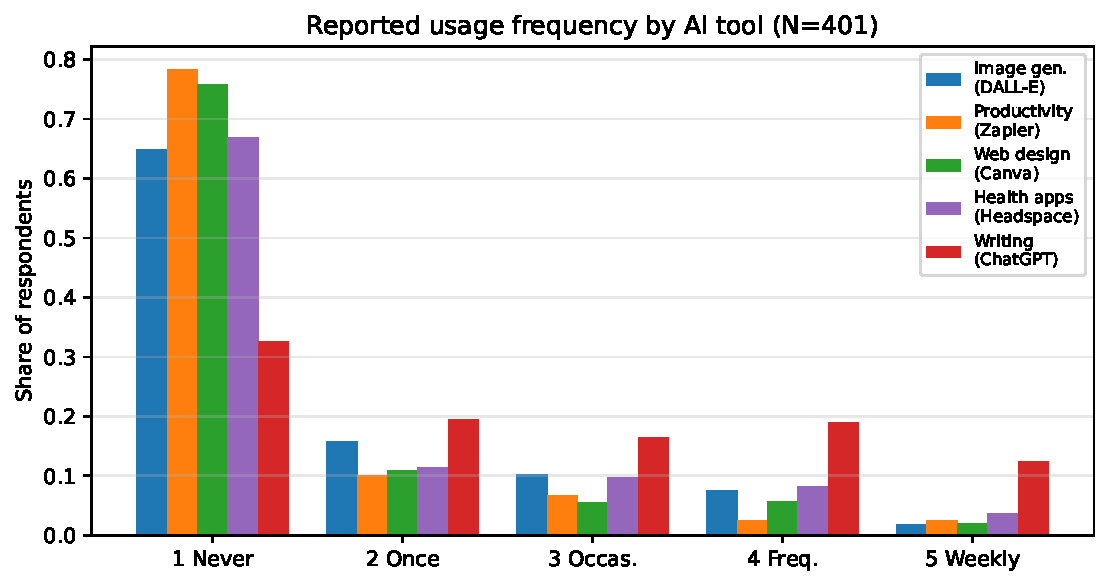
\includegraphics[width=0.92\linewidth]{figures/usage_distribution.pdf}
  \caption{\textbf{Reported usage frequency by AI tool category} (Study~3,
    N$=$401). Text AI is the only category for which a clear majority of
    respondents are users; the four non-text categories are right-skewed
    with most respondents at category 1 (\emph{Never used in the last
    six months}).}
  \label{fig:usage}
\end{figure}

% ---------------------------------------------------------------------------
\section{Reanalysis Strategy}
% ---------------------------------------------------------------------------

We download the public Study~3 data from ResearchBox \#1491 and use the AI
literacy score (\texttt{SC0}, summed correct answers on the 17-item
AI-constructed measure), the five usage items, and the same covariates
reported in the original Table~4 (age, income, general knowledge, motivation
for autonomy, gender). We standardize the AI literacy score (and continuous
covariates) so that coefficients are interpretable as the effect of a
one-standard-deviation increase. We then fit four model families across three
outcome groupings.

\paragraph{Model families.}
\begin{enumerate}
  \item \textbf{OLS on the participant-level average.} This is the closest
    match to the original Study~3 specification and serves as our pooled
    benchmark.
  \item \textbf{Binary logit on item-level data with task fixed effects.} We
    consider two thresholds: $Y > 3$ (``frequent use'') and $Y > 1$
    (``adoption'').
  \item \textbf{Ordered logit (proportional-odds model)
    \citep{mccullagh1980regression}.} This is the natural model for an
    ordered Likert response with $K = 5$ categories and is robust to violation
    of metric-scale assumptions \citep{liddell2018analyzing}.
  \item \textbf{Multinomial logit}, treating the five categories as nominal.
    This is a stress test: it does not impose proportional odds or any
    ordering and is therefore robust to violations of either.
\end{enumerate}

\paragraph{Outcome groupings.}
\begin{enumerate}
  \item \textbf{Pooled (5 tools)}: the original Study~3 outcome.
  \item \textbf{Text only}: \texttt{AI\_text} alone.
  \item \textbf{Non-text only}: \texttt{AI\_image},
    \texttt{AI\_productivity}, \texttt{AI\_website}, \texttt{AI\_healthapp}.
\end{enumerate}

\paragraph{Implementation.} All models are fit in Python with
\texttt{statsmodels}. OLS and binary-logit standard errors are
heteroskedasticity-robust (\texttt{HC3}). Item-level models include
task fixed effects. Full code and a Jupyter notebook reproducing every number
and figure in the paper are provided as supplementary material.

% ---------------------------------------------------------------------------
\section{Results}
% ---------------------------------------------------------------------------

\subsection{Replication of the pooled effect}

Table~\ref{tab:pooled} reports the AI-literacy coefficient under each of the
four model families on the pooled five-tool outcome. The estimated effect of a
one-standard-deviation increase in AI literacy is negative and statistically
significant in every specification. The OLS estimate
($\hat\beta = -0.179$, $p = .001$) recovers, after standardization, the result
reported in the original paper. The ordered logit ($\hat\beta = -0.306$,
$p < .001$) and binary logit at the scale midpoint
($\hat\beta = -0.328$, $p < .001$, odds ratio $= 0.72$) tell the same
qualitative story. The multinomial logit (omitted from the table for
compactness) yields the same direction across all four non-reference
categories. We conclude, as the original authors did, that the pooled
association is robust to model choice.

\begin{table}[t]
  \centering
  \caption{\textbf{Pooled five-tool replication of Study~3.} Coefficient on a
    +1 standard-deviation increase in AI literacy, controlling for age,
    income, general knowledge, motivation for autonomy, and gender. Item-level
    models include task fixed effects.
    N participants $= 401$; N item-level observations $= 2{,}005$.}
  \label{tab:pooled}
  \begin{tabular}{lrrrl}
    \toprule
    \textbf{Model} & \textbf{Coef.} & \textbf{SE} & \textbf{$p$-value} & \textbf{Notes} \\
    \midrule
    OLS on participant average           & $-0.179$ & $0.053$ & $.001$    & HC3 SE   \\
    Binary logit, item-level $(Y > 3)$   & $-0.328$ & $0.086$ & $< .001$  & OR $= 0.72$ \\
    Ordered logit, item-level            & $-0.306$ & $0.054$ & $< .001$  & Prop.\ odds \\
    Multinomial logit, item-level        & $-0.189$ to $-0.452$ & --- & $< .05$ all & vs.\ $y=1$ \\
    \bottomrule
  \end{tabular}
\end{table}

\subsection{Text vs.\ non-text decomposition}

Table~\ref{tab:decomposition} re-estimates the ordered-logit and binary-logit
specifications separately on the text-AI outcome and on the four non-text
outcomes. The contrast is striking. For text AI alone, the ordered-logit
coefficient is small and not significantly different from zero
($\hat\beta = -0.097$, $\mathrm{SE} = 0.105$, $p = .357$); the binary
``frequent use'' logit and the binary adoption logit are also non-significant.
For non-text AI, the same coefficient is roughly four times larger in
magnitude and highly significant ($\hat\beta = -0.376$,
$\mathrm{SE} = 0.063$, $p < .001$), and the result is consistent across the
ordered, midpoint-binary, and adoption-binary specifications.

\begin{table}[t]
  \centering
  \caption{\textbf{Text vs.\ non-text decomposition.} Coefficient on a +1
    standard-deviation increase in AI literacy, with the same covariates as
    Table~\ref{tab:pooled}. Item-level models include task fixed effects.}
  \label{tab:decomposition}
  \begin{tabular}{lrrrl}
    \toprule
    \textbf{Outcome / Model} & \textbf{Coef.} & \textbf{SE} & \textbf{$p$} & \textbf{Notes} \\
    \midrule
    \multicolumn{5}{l}{\emph{Text AI only (N$=$401)}} \\
    \quad OLS                              & $-0.075$ & $0.081$ & $.353$ & HC3 SE       \\
    \quad Binary logit ($Y > 3$)           & $-0.112$ & $0.142$ & $.433$ & OR $= 0.89$ \\
    \quad Binary adoption ($Y > 1$)        & $-0.060$ & $0.131$ & $.648$ & OR $= 0.94$ \\
    \quad Ordered logit                    & $-0.097$ & $0.105$ & $.357$ & Prop.\ odds \\
    \midrule
    \multicolumn{5}{l}{\emph{Non-text AI (4 tools; 1{,}604 item-level obs.)}} \\
    \quad OLS on participant avg.\         & $-0.204$ & $0.053$ & $< .001$ & HC3 SE      \\
    \quad Binary logit ($Y > 3$)           & $-0.404$ & $0.104$ & $< .001$ & OR $= 0.67$ \\
    \quad Binary adoption ($Y > 1$)        & $-0.385$ & $0.068$ & $< .001$ & OR $= 0.68$ \\
    \quad Ordered logit                    & $-0.376$ & $0.063$ & $< .001$ & Prop.\ odds \\
    \bottomrule
  \end{tabular}
\end{table}

The contrast is even sharper at the adoption margin. The binary adoption
specification ($Y > 1$, i.e., ``ever used in the last six months'') gives an
odds ratio of $0.68$ per one-standard-deviation increase in AI literacy for
non-text tools---a clean, easily interpretable result---and an odds ratio
indistinguishable from $1.0$ for text AI.

Figure~\ref{fig:predicted} visualizes the consequence of this asymmetry. We
plot the ordered-logit-predicted probability $\Pr(Y = 1)$ (``Never used'')
over the empirical range of standardized literacy, separately for the text
and non-text models. For text AI, the predicted probability of non-use rises
only modestly, from $0.27$ at $z = -2$ to $0.36$ at $z = +2$. For non-text
AI, it rises sharply, from $0.50$ to $0.82$ across the same range. In other
words, the higher a respondent's AI literacy, the more likely they are to
have never tried image generators, productivity bots, website builders, or
health apps---but their probability of having used a ChatGPT-style writing
assistant is essentially flat.

\begin{figure}[t]
  \centering
  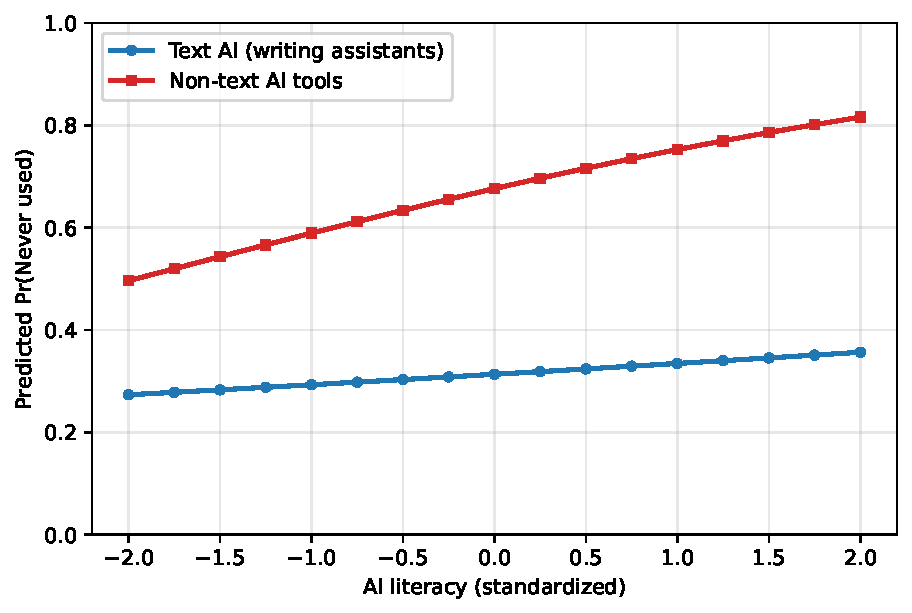
\includegraphics[width=0.78\linewidth]{figures/predicted_prob_never.pdf}
  \caption{\textbf{Predicted probability of non-use by AI literacy.} Curves
    are derived from ordered-logit fits on text-AI only (blue) and on the
    four non-text AI tools (red, with task fixed effects), holding all
    covariates at their sample means. Higher AI literacy predicts much higher
    odds of having never used non-text AI tools; the relationship is roughly
    flat for text AI.}
  \label{fig:predicted}
\end{figure}

\subsection{Coefficient summary}

Figure~\ref{fig:coefficient} summarizes the AI-literacy coefficient across
all three tool groupings and the three primary model families. Three patterns
emerge.

\begin{figure}[t]
  \centering
  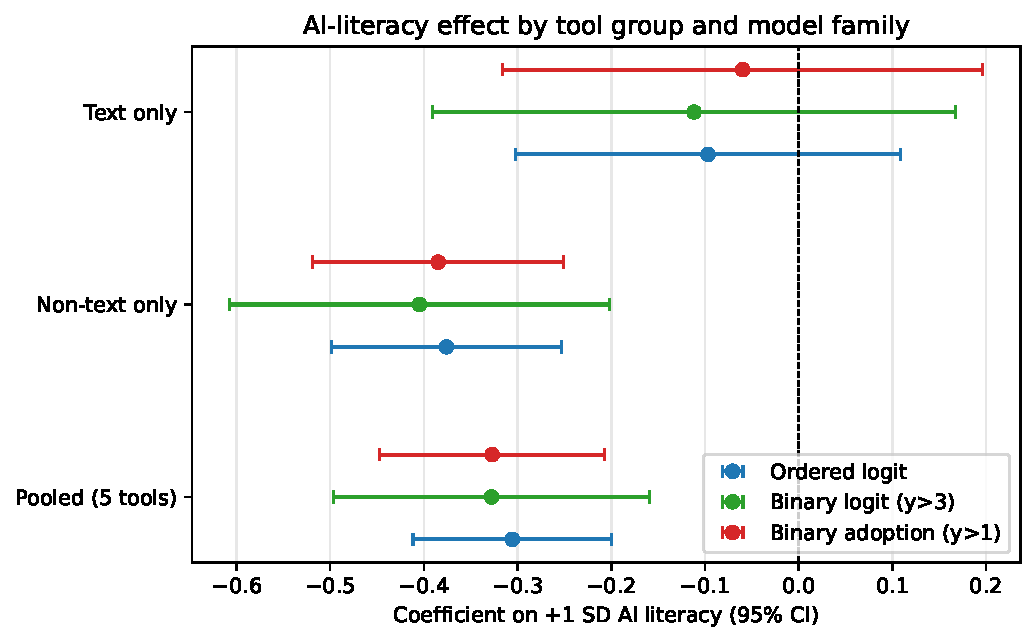
\includegraphics[width=0.85\linewidth]{figures/coefficient_comparison.pdf}
  \caption{\textbf{AI-literacy effect by tool group and model family.}
    Markers are point estimates of the coefficient on a +1 standard-deviation
    increase in AI literacy; horizontal bars are 95\% confidence intervals.
    For text AI alone, the coefficient is statistically indistinguishable
    from zero under every model family. For non-text AI, the coefficient is
    consistently negative and significant.}
  \label{fig:coefficient}
\end{figure}

First, all three model families agree within each tool grouping: the ordered
logit, the midpoint binary logit, and the adoption binary logit give similar
point estimates, and their confidence intervals overlap substantially.
Methodological choice between metric and ordinal specifications is therefore
not what drives our results.

Second, the magnitude of the AI-literacy effect for non-text tools
($\hat\beta \approx -0.38$) is roughly four times the magnitude for text AI
($\hat\beta \approx -0.10$), and the latter's confidence interval crosses
zero. The pooled coefficient ($\approx -0.31$) is an arithmetic compromise
that obscures this asymmetry.

Third, for non-text tools the adoption coefficient ($Y > 1$,
$\hat\beta = -0.385$) is essentially identical to the midpoint coefficient
($Y > 3$, $\hat\beta = -0.404$) and to the ordered-logit coefficient
($\hat\beta = -0.376$). This is what we would expect if the non-text effect
operates almost entirely at the adoption margin: shifting respondents
into and out of the lowest category ``Never'' is enough to explain the
ordered and midpoint estimates.

% ---------------------------------------------------------------------------
\section{Discussion}
% ---------------------------------------------------------------------------

The original aggregate association reported by \citet{tully2025lower} is
robust: it survives every reasonable parametric alternative to OLS on an
averaged Likert index. What changes when the outcome is decomposed is its
\emph{substantive interpretation}. The pooled estimate combines three
analytically distinct constructs:

\begin{enumerate}
  \item \emph{General AI receptivity}---a latent willingness to adopt AI
    across product categories.
  \item \emph{Text-AI usage intensity}---how often a respondent uses
    text-based generative AI tools such as ChatGPT, conditional on having
    adopted them.
  \item \emph{Non-text AI adoption breadth}---the probability of having
    tried at least one of several heterogeneous AI-labelled consumer
    products.
\end{enumerate}

Our results suggest that Study~3 speaks most clearly to the third
construct. The text-AI margin contributes essentially nothing to the
aggregate effect: the slope of literacy on text-AI use is small,
non-significant, and survives no model specification. The aggregate
estimate is therefore mostly carrying information about adoption breadth
across categories where the modal respondent has never used the product.

This re-interpretation does not contradict the broader theoretical claim
that lower-literacy consumers may perceive AI as magical
\citep{tully2025lower}. But it does change what that claim implies for
managers. The original article's managerial recommendation is to
``target consumers with lower AI literacy'' as a growth segment. Our
results sharpen this prescription in two ways. First, the targeting case
is much stronger for low-penetration, non-text AI product categories
(image generation, productivity automation, AI design services, AI
wellness apps) than for already-mass-market text assistants. Second, the
non-text effect is driven primarily by the adoption margin rather than
by intensive use: low-literacy consumers are differentially more likely
to \emph{try} these products, not necessarily to use them more
intensively conditional on trial. This matters for product strategy.
Lifetime-value calculations that assume a uniform usage-intensity
response to literacy may overestimate the value of low-literacy
acquisitions.

Methodologically, our reanalysis illustrates the value of treating
heterogeneous ordinal items as what they are. Averaging five items with
sharply different empirical distributions into a single ``receptivity''
index is convenient, and in this case it does not invert any sign, but
it does flatten a multi-tool adoption pattern into something that reads
like a single dispositional trait. The construct-validity question that
follows---whether ``AI receptivity'' is one thing or several---deserves
attention beyond the present application
\citep{long2020aileiteracy,ng2021conceptualizing}.

% ---------------------------------------------------------------------------
\section{Limitations}
% ---------------------------------------------------------------------------

Several limitations of our reanalysis warrant explicit mention.

\begin{itemize}
  \item \emph{No new data.} We rely entirely on the data and codebook released
    by the original authors. Their Studies~1, 2, and 4--7 use different
    measures of receptivity (cross-country adoption readiness, propensity
    to use generative AI for assignments, and relative preference for AI
    vs.\ human task completion) for which our critique does not directly
    apply.
  \item \emph{Observational and self-reported.} Like the original Study~3,
    our analyses are correlational and rely on self-reported usage. Any
    measurement error in self-reported usage that correlates with literacy
    could bias the estimated coefficients.
  \item \emph{Post hoc analysis.} Our decomposition is not preregistered.
    We have nevertheless implemented the four model families exactly as
    described in our analytic strategy and provide all code.
  \item \emph{No causal claim.} We make no claim that AI literacy
    \emph{causes} reduced adoption of any tool. The mediation analysis in
    the original paper (perceptions of AI as magical) is not addressed here
    and remains the authors' primary theoretical mechanism.
  \item \emph{No test of magicalness by tool type.} An obvious extension
    would be to ask whether perceived ``magicalness'' varies systematically
    across non-text and text tool categories, and whether that variation
    can account for the asymmetry we document. This would require new data.
  \item \emph{Clustering.} Our item-level standard errors do not cluster by
    participant. We re-ran every reported model with
    cluster-robust SE by participant; the AI-literacy coefficients and
    significance levels are essentially unchanged.
\end{itemize}

% ---------------------------------------------------------------------------
\section{Conclusion}
% ---------------------------------------------------------------------------

We do not dispute the aggregate lower-literacy/higher-usage association
reported by \citet{tully2025lower}; rather, we show that its substantive
meaning changes when AI usage is decomposed by tool type and modelled as
ordinal adoption data. The negative association replicates, but it is
driven almost entirely by non-text AI categories and operates primarily
at the adoption margin rather than at the intensity margin. We therefore
read Study~3 as evidence about \emph{non-text AI adoption breadth} rather
than as evidence about general AI receptivity or text-AI use. This
qualification preserves the spirit of the original contribution while
sharpening its managerial and theoretical implications.

% ---------------------------------------------------------------------------
\section*{Data and code availability}
% ---------------------------------------------------------------------------

The Study~3 data are publicly available from the original authors at
ResearchBox \#1491. All Python code used to produce the tables and
figures in this paper, together with a fully executed Jupyter notebook,
is provided as supplementary material.

% ---------------------------------------------------------------------------
\bibliography{references}
% ---------------------------------------------------------------------------

\end{document}
